\documentclass[../tb_report.tex]{subfiles}

\begin{document}

\chapter{Proof of space}
\label{ch:pospace}

\section{Introduction}

La \emph{preuve d'espace} (ou \emph{proof of space} en anglais) est un algorithme de consensus similaire à la preuve de travail à la différence qu'au lieu d'effectuer des calculs de manière continue pour trouver une preuve satisfaisant les conditions de la difficulté de la blockchain, les mineurs appelés farmers avec \emph{PoSpace} vont trouver des preuves à partir d'un challenge grâce à une certaine quantité de données allouées sur le disque dur. 

Il existe principalement deux constructions pour faire du proof of space : une basée sur l'inversion de fonctions de hachage en utilisant le compromis temps-mémoire de Hellman \cite{DBLP:conf/asiacrypt/AbusalahACKPR17} et une basée sur des \emph{hard-to-pebble graphs} \cite{DBLP:conf/crypto/DziembowskiFKP15}.

Pour ce travail, il a fallu faire un choix d'un algorithme à implémenter. Ce choix c'est porté sur la construction des compromis temps-mémoire car il y plus de ressources disponibles. De plus, la construction des graphs de type \emph{hard-to-pebble} s'avère être trop compliquée pour un travail comme celui-ci, c'est aussi pourquoi elle a été écartée.

Ce chapitre explique le fonctionnement général du protocole principalement tiré de la blockchain Chia. Les détails d'implémentation sont décrits dans le chapitre suivant [\ref{ch:realisation}].

\section{Résumé du protocole}

Dans un premier temps, les données sont générées par le farmer dans une étape appelée \textbf{plotting}. Ce sont des données pseudo-aléatoires qui ne représentent rien de particulier. D'autres algorithmes pour stocker des données utiles existent comme \emph{proof of catalytic space} ou \emph{proof of replication} utilisés dans la blockchain \href{https://filecoin.io/}{Filecoin} par exemple.

En suite, un farmer peut prouver qu'il a bien les données qu'il dit avoir stockées en trouvant une ou plusieurs preuves répondant à un challenge donné. C'est l'étape du \textbf{farming}.

Lors de la \textbf{vérification}, le vérificateur récupère la prevue est à partir de celle-ci, recalcule le challenge et vérifie s'il correspond à celui envoyé précédemment.

Ainsi, on peut considérer \emph{proof of space} comme est un protocole dans lequel nous avons :

\begin{enumerate}
  \item un vérificateur qui envoie un challenge à un farmer et
  \item un farmer qui peut prouver au vérificateur qu'il a bien alloué la quantité d'espace spécifiée à un instant $t$.
\end{enumerate}

\begin{figure}[H]
  \centering
  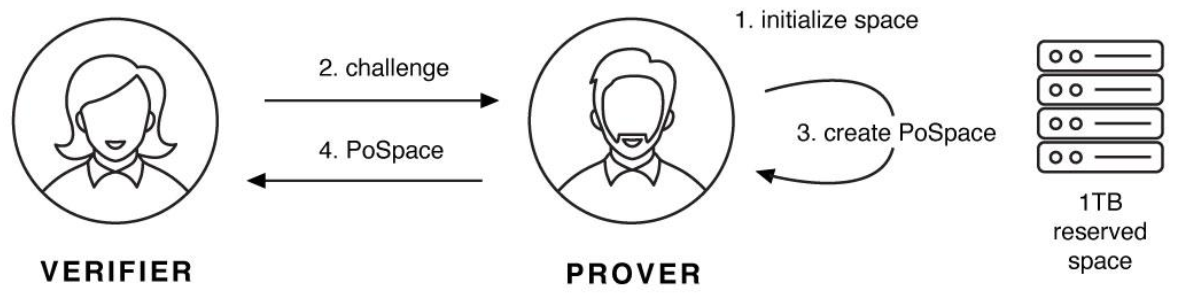
\includegraphics[width=\textwidth]{images/pospace.png}
  \caption{Diagramme du protocole \emph{proof of space} montrant les différentes étapes. Tiré de \cite{chia:consensus}}
\end{figure}

\section{Plotting}

Le plotting est un procédé non-interactif dans le lequel le farmer va créer les données qui seront stockées et qui permettront de trouver les preuves d'espace liées aux challenges. Ce procédé peut être long, cela peut prendre de plusieurs heures à plusieurs jours suivant la quantité de données allouées.

La construction de cette preuve d'espace est basée sur la construction de Chia \cite{chia:construction}, elle-même basée sur l'inversion de fonctions de hachage \cite{DBLP:conf/asiacrypt/AbusalahACKPR17}. Elle a cependant été simplifiée pour pouvoir être réalisée dans le temps imparti de ce travail. 

Le principe est le suivant: soit une fonction modélisée comme un oracle aléatoire $f: [N] \rightarrow [N]$, où $N=2^k$ et $k$ étant le \emph{space parameter}, le farmer doit être capable de l'inverser rapidement. Pour ce faire, on peut imaginer que le farmer précalcule la table de la fonctions et la trie par rapport à la valeur de sortie. Ainsi, lorsqu'un challenge est donné au farmer, il a simplement à regarder dans la table des valeurs de sortie par une recherche dichotomique et renvoyer l'entrée associée comme avec une lookup-table. Par exemple, on peut modéliser $f$ comme une fonction de hachage cryptographique et la table serait: $f(x) = H(n\|x)$, avec $n$ un nonce aléatoire. \cite{chia:construction}

\begin{figure}[H]
  \centering
  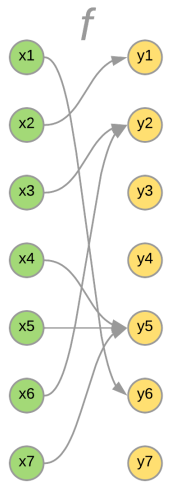
\includegraphics[width=3.5cm]{images/pospace_1.png}
  \caption{Table simplifiée, tiré de \cite{chia:construction}}
\end{figure}

Cependant, à cause d'un compromis temps-mémoire, il est possible de faire une attaque de \emph{Hellman} avec laquelle il est possible de stocker uniquement $N^{1/2}$ valeurs et les autres $N^{1/2}$ valeurs seront calculées à la demande. Pour éviter un maximum ce problème, il faut rendre la fonction $[N] \rightarrow [N]$ difficile à calculer pour rendre l'initialisation plus longue et réduire le compromis temps-mémoire mais elle doit rester facilement inversible, ceci pour forcer les farmers à stocker l'entièreté de la table. \cite{chia:construction}

Pour rendre plus difficile à calculer vers l'avant, on peut modéliser une nouvelle fonction $f(x_1)=f_2(x_1,x_2)$, où $f_2(x_1,x_2)=H(x_1\|x_2)$ avec la condition que $f_1(x_1)=f_1(x_2)+1$, avec $f_1$ une autre fonction de hachage. Ainsi, à partir d'un challenge $z$, le farmer doit trouver les valeurs $x_1$ et $x_2$. Et comme la fonction $f$ n'est pas facilement calculable, le farmer doit stocker toutes les tables pour pouvoir répondre rapidement. Cette construction, illustrée ci-dessous, est toujours proie au attaques de Hellman mais il suffi de rajouter des tables pour la rendre encore plus lente à calculer. \cite{chia:construction}

\begin{figure}[H]
  \centering
  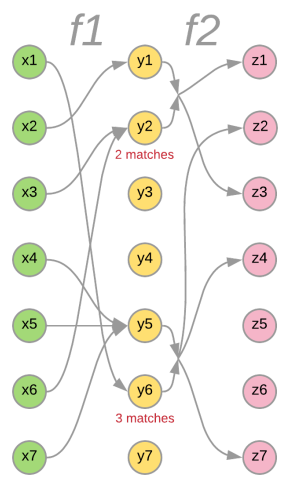
\includegraphics[width=6cm]{images/pospace_2.png}
  \caption{Table améliorée, tiré de \cite{chia:construction}}
\end{figure}

Ainsi, le farmer choisi un nombre $k$, le \emph{space parameter} pour définir combien il souhaite allouer d'espace. La quantité de données finale sera exponentielle par rapport à ce nombre $k$. Le temps de la génération dépend de la puissance de l'ordinateur effectuant le plotting puisqu'il s'agit principalement d'exécution de fonctions de hachage comme vu précédemment. C'est le CPU qui sera beaucoup sollicité durant cette étape. 

Pour ce travail, le nombre de tables sera de 4 pour simplifier l'implémentation contre 7 pour Chia. Chaque table contiendra $2^k$ entrées et chaque entrée d'une $\textsf{table}_i$ pointera vers 2 entrées dans la $\textsf{table}_{i-1}$. La première table quant à elle contiendra ce qu'on appellera les \emph{x-values}. Ce sont simplement des nombres entiers de $0$ à $2^k-1$. Ainsi. une preuve d'espace correspond à 8 \emph{x-values} ($2^{\textsf{nombre de table} - 1} = 2^3 = 8$). A noter que ce processus à besoin de plus d'espace de stockage que souhaité pour le plot final car il générera des données qui seront ensuite nettoyées et compressées. La génération des tables occupera plus de place que le plot final. On supprimera ensuite les sorties des fonctions de hachages de chaque table intermédiaire pour ne stocker plus que les index dans la 1ère table pour chaque table.

Une fois les 4 tables générées, on peut commencer à faire du \textbf{farming}.

Les détails de l'implémentation et des choix réalisés sont décrits dans le chapitre suivant.

\section{Farming}

Le \emph{farming} est le processus dans lequel le farmer reçoit un challenge et produit une preuve composé de 8 x-values pour démontrer qu'il a bien alloué l'espace indiqué. Le challenge est une valeur de 256 bits (un hash par exemple). Pour ce faire, le farmer regarde dans la dernière table de son plot si $\underset{k}{\mathrm{trunk}}(\mathrm{Chall})=\underset{k}{\mathrm{trunk}}(\mathrm{table_4}[i])$, pour $i \in \{0,1,\dots,2^k-1\}$. S'il trouve un correspondance, le farmer parcours les tables dans le sens inverse, de la 4 à la 1, pour retrouver les x-values puisque $\mathrm{table_4}[i]=f_4(x_1,x_2,\dots,x_8)$. Il renvoie ensuite les 8 valeur au vérificateur.

Dans le cas d'une blockchain, le système est non-interactif. La preuve doit pouvoir être vérifiée par n'importe qui à tout moment sans avoir besoin de demande quoi que ce soit au farmer en question. Pour ce faire le challenge doit être généré à partir d'un élément public, par exemple le hash du dernier bloc de la chaîne.

\section{Vérification}

La vérification consiste à valider une preuve donnée par un farmer. Elle est plutôt simple puisqu'il suffit de recalculer les 4 tables avec uniquement les 8 x-values de la preuve. Ce qui peut être réalisé rapidement car ce n'est que $8 \times 2 - 1 = 15$ exécutions de fonction de hachage qui peuvent être faite en parallèle. Le vérificateur check ensuite la valeur calculée avec le challenge.

\section{Sécurité et attaques}

Comme vu dans le chapitre sur les protocoles de consensus, \emph{proof of space} a des avantages écologiques puisque le calcul n'est réalisé qu'une fois au début lors de la génération du plot. Cela signifie que la génération de preuve ne requiert que très peu de puissance calcul et que par conséquent elle peut être exécutée rapidement à la différence de proof of work. Cela implique qu'un attaquant peut forger des blocs en avance, générer leur preuve respective et les broadcasté sur le réseau. Si ces blocs sont valides ils pourraient être acceptés par le réseau qui se base automatiquement sur la plus longue chaîne de blocs. Il y aurait du coup la possibilité pour des attaquant d'effectuer des actes de double dépenses.

Pour palier à ce problème, la blockchain Chia utilise des preuves de temps (proofs of time en anglais) basées sur des \emph{Verifiable Delay Functions} afin de vérifier qu'un certain c'est réellement écoulé et empêcher la création de bloc à l'avance.

\end{document}